% Chapter Template

\chapter{The nuclear spin qubit with an electric dipole transition} % Main chapter title

\label{Chapter3} 

\noindent\hrulefill
\vspace{0.5cm} %\hspace{2cm}
%\small
\begin{flushright}
        ``\emph{I’ve yet to see any problem, however complicated, which when you looked at it the right way didn’t become still more complicated.}"
\\ 
--Poul Anderson, \textit{Call Me Joe} \\
%“The most complicated skill is to be simple.” ―Dejan Stojanovic
\end{flushright}

\vspace{0.5cm}


\noindent\hrulefill
\vspace{0.5cm} %\hspace{2cm}
\\
%\small
\hangindent=4cm
%\noindent
\\
The nuclear spin state of a phosphorus donor in isotopically enriched silicon-28 is an excellent host to store quantum information in the solid state. The spin's insensitivity to electric fields yields a solid-state qubit with record coherence times but also renders coupling to other quantum systems very challenging. In this chapte, we describe how to generate a strong electric dipole ($>100$ D) at microwave frequencies for the nuclear spin. This is achieved by applying a magnetic drive to the electrically controlled flip-flop qubit. The dipole then allows for coupling to microwave resonators, with a vacuum Rabi splitting of the order of 1 MHz. This work brings the $^{31}$P nuclear qubit into the realm of hybrid quantum systems and opens up new avenues in quantum information processing.
\\ \\
\scriptsize
\hangindent=4cm
The work presented in this chapter has been published in:\\
G. Tosi, F. A. Mohiyaddin, \textbf{S. Tenberg}, A. Laucht, A. Morello. ``Robust electric dipole transition at microwave frequencies for nuclear spin qubits in silicon.'' \textit{Physical Review B} vol. 98, 075313 (2018).\\
\\
\footnotesize
\hangindent=4cm
\textbf{The author acknowledges G. Tosi for the conception of the idea and the bulk of the simulation work and F. A. Mohiyaddin for tight-binding simulations and electric modelling.}\\

%\vspace{0.5cm}

\noindent \hrulefill
\clearpage

\normalsize


\section{Introduction}

The nuclear spin of a phosphorus donor in silicon has long been the subject of much study in the context of solid-state quantum information processing, either as a qubit cell for large-scale quantum processors \cite{Kane1998,OGorman2016,Hill2015}, or a memory for long-lived quantum information storage \cite{Morton2008,Freer2017}. Whether in ensemble form \cite{Saeedi2013} or as individual qubit \cite{Muhonen2014}, the $^{31}$P nuclear spin has record-long coherence times, thanks to its insensitivity to electric fields and the possibility to drastically reduce magnetic environmental noise by hosting it in isotopically pure $^{28}$Si \cite{Itoh2014}. However, it cannot trivially be coupled to other quantum systems, and therefore all quantum computing proposals so far impose short interaction distances and slow quantum gate operations \cite{Kane1998,OGorman2016,Hill2015}.

In the hybrid approach to quantum information processing \cite{Xiang2012}, different quantum systems interact in a large architecture that benefits from the best properties of each system, which are often coupled together via microwave resonators. In order to couple to individual spin qubits, the resonator vacuum field can be enhanced by shrinking its dimensions in the vicinity of the spin qubit, thereby enhancing the spin-photon coupling rate \cite{Tosi2017,Jenkins2016,Haikka2017,Sarabi2018}. However, having a Zeeman splitting in the radio-frequency range and a null electric dipole, phosphorus nuclear-spins do not interact naturally with microwave resonators.

The artificial creation of electric dipole transitions has been proposed for different spin systems \cite{Pioro-Ladriere2008,Shi2012,Russ2017,Salfi2016,Tosi2017} as a way to facilitate scalability. The challenge here is how to make the spin drivable by electric fields without making it too susceptible to electrical noise, which can be significant in nanoscale electronic devices. In this chapter, we show how to engineer a strong electric dipole transition at microwave frequencies for the nuclear spin, based on the flip flop qubit and our finding from chapter \ref{Chapter2}, by applying an oscillating magnetic field to the nucleus while the electron is shared between the donor and a quantum dot defined at the Si/SiO$_2$ interface \cite{Calderon2009,Veldhorst2014, Tosi2017,Harvey-Collard2017}. While the admixture of spin and charge states can potentially make the system very sensitive to electric noise, we show that the nuclear spin precession frequency and electric dipole strength can be rendered highly immune to electrical noise by a peculiar choice of spin-charge hybridization, same than for the flip flop qubit. By providing a robust coupling between the nuclear spin and electric fields, our scheme opens up new avenues to couple $^{31}$P qubits to other quantum systems, including microwave resonators, superconducting qubits, or simply other nuclear spins but at distances and with speeds that had not been anticipated so far.


\section{Second-order Raman drive of a $^{31}$P nuclear spin} \label{sec:Raman}


\begin{figure}
\centering
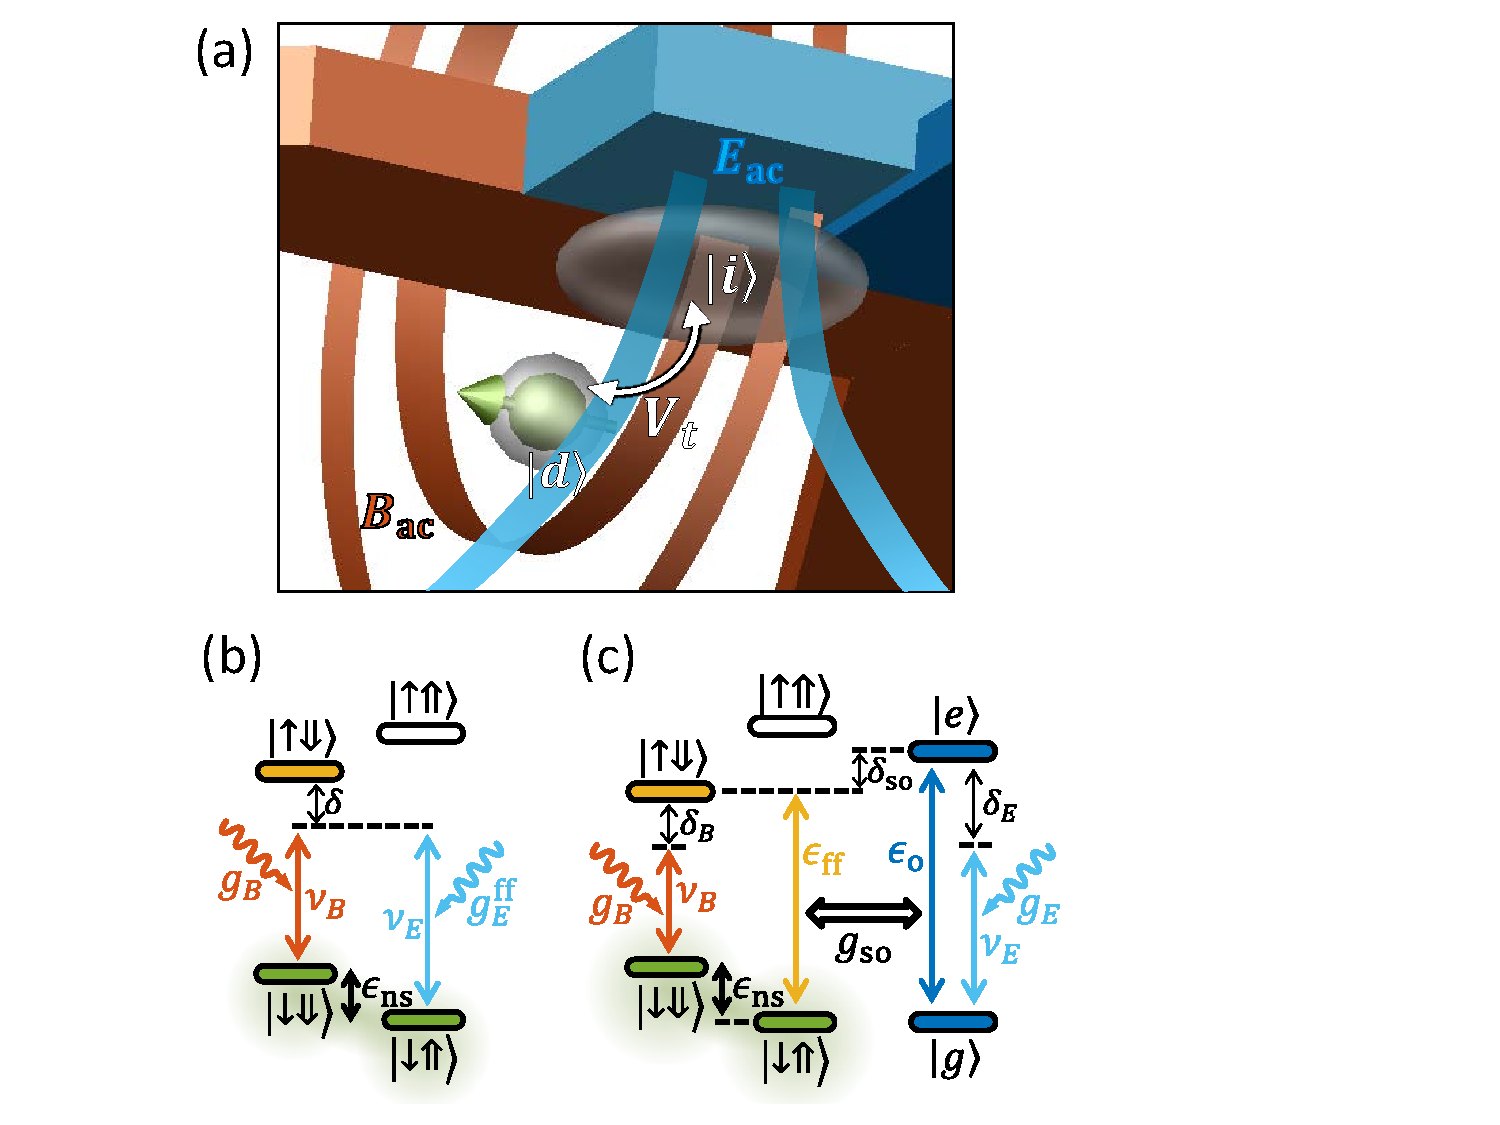
\includegraphics[width=0.8\columnwidth]{fig1_Raman_v5}
\caption[Nuclear Raman transition]{\textbf{Nuclear Raman transition. a}, Components of a Raman-enabled Si:P nuclear electric dipole transition. The electron  spatial wavefunction (transparent gray) is shared between an interface-dot, $|i\rangle$, and a donor-bound state, $|d\rangle$, which are coupled by a tunnel rate $V_t$. Metallic gates (blue) on top of SiO$_2$ dielectric (not shown) control the electron charge state via a static vertical field $E_{\rm dc}$, and can introduce an oscillating electric field $E_{\rm ac}$. In a circuit-Quantum Electrodynamics setup, the electrostatic gate can be replaced by the inner conductor of a microwave resonator, and $E_{\rm ac}$ by the vacuum field of such resonator. A nearby broadband antenna \cite{Dehollain2014} (brown) provides the magnetic drive $B_{\rm ac}$. 
\textbf{b} Simplified energy level diagram for Raman-drive of the Si:P nuclear-spin qubit, with energy splitting $\epsilon_{\rm ns}$. The second-order Raman drive is obtained by combining the microwave electric and magnetic drives, having frequencies $\nu_B$ and $\nu_E$, respectively, and coupling rates $g_B$ and $g_E^{\rm ff}$, respectively. The drive is detuned by a frequency $\delta$ from the $\ket{\uparrow \Downarrow}$ state. 
\textbf{c} Expanded energy diagram including the charge states $\ket{g}$ and $\ket{e}$.
}
\label{fig:Raman}
\end{figure}


The base of our proposal for an electrically accessible nuclear qubit is the flip flop qubit, as described in chapter \ref{Chapter2}, with the Hamiltonian $\mathcal{H}_{\rm ff}$ from eq. \eqref{eq:H_ff_ge}. 

The electron and nuclear spins can be coherently driven by conventional magnetic resonance transitions using oscillating magnetic fields at microwave \cite{Pla2012} and radio frequencies \cite{Pla2013} (see chapter \ref{sec:magRes}). In particular, the nuclear spin transition frequency when the electron spin is $\ket{\downarrow}$ (i.e. the $\ket{\downarrow \Uparrow} \leftrightarrow \ket{\downarrow \Downarrow}$ transition) is:
\begin{equation} \label{eq:epsilon_ns}
\epsilon_{\rm ns}(A) = \gamma_nB_0 + A/2.
\end{equation}


Now we show how the flip-flop transition provides a way of controlling the nuclear spin state without any radiofrequency field, by using instead two microwave-frequency excitations, one of which is electric, as illustrated in figure \ref{fig:Raman}a. This has important advantages over magnetic-only schemes \cite{Morton2008,Freer2017}, since it allows coupling a nucleus to the vacuum electric field of a microwave cavity, or to another nucleus similarly equipped with an electric dipole, as we will show below. The key idea is to combine the electrical drive of the flip-flop transition with an additional magnetic drive $B_{\rm ac}\cos(2\pi\nu_Bt)$, perpendicular to the static $B_0$ (Fig \ref{fig:Raman}a), where the Hamiltonian is 

\begin{equation}
\mathcal{H}_{\rm ESR}=B_{\rm ac}\cos(2\pi\nu_Bt)\left(\gamma_e S_x-\gamma_n I_x\right)
\end{equation}

which gives the full nuclear qubit Hamiltonian
\begin{equation}
\mathcal{H}_{\rm ns}=\mathcal{H}_{\rm ff}+\mathcal{H}_{\rm E}+\mathcal{H}_{\rm ESR}.
\end{equation}

 This magnetic drive is the conventional electron spin resonance (ESR) transition, that couples the electron spin states $\lvert\downarrow\Downarrow\rangle$ and $\lvert\uparrow\Downarrow\rangle$ at a rate:
\begin{equation}
g_{B}=\bra{\downarrow}\mathcal{H}_{\rm ESR}\ket{\uparrow}= \gamma_eB_{\rm ac}/4.
\end{equation}

Combining these two driving fields results in a process analogous to a Raman transition \cite{Kok2010}, as shown in Fig. \ref{fig:Raman}b: with the electron in the ground spin state $\ket{\downarrow}$, the AC electric and magnetic fields drive the nuclear-spin ``up'', $\lvert\downarrow\Uparrow\rangle$, and ``down'', $\lvert\downarrow\Downarrow\rangle$, states, respectively, to a virtual level detuned from the $\lvert\uparrow\Downarrow\rangle$ state by $\delta\gg g_B,g_E^{\rm ff}$. As a result, the nuclear spin is driven via a second order process, with minimal excitation of the electron spin, at a rate:

\begin{eqnarray}
\label{eq:g_E^ns_simple}
g_E^{\rm ns} & = & \frac{\left|\bra{\Downarrow \downarrow g} H_{ns} \ket{\Uparrow \downarrow g} \bra{\Downarrow \downarrow g} H_{ns} \ket{\Uparrow \downarrow g} \right|}{E_{\Downarrow \downarrow g}-E_{\Uparrow \downarrow g}}\\
& = & \frac{g_B g_E^{\rm ff}}{\delta}.
\end{eqnarray} 

This can be interpreted such that the microwave magnetic drive $B_{\rm ac}$ creates an electric dipole transition for the nuclear spin mediated by the flip-flop qubit, with strength:

\begin{equation}
p_E^{\rm ns} = \frac{4 g_E^{\rm ns}}{E_{\rm ac}} = \frac{4 g_B g_{E}^{\rm ff}}{E_{\rm ac} \delta}.
\label{eq:pns}
\end{equation}

The coupling $g_{E}^{\rm ff}$ between the flip-flop qubit and the AC electric field corresponds to a strong electric-dipole flip-flop transition ($\sim80$~Debye, assuming $\delta_{\rm so}=10g_{\rm so}$). Combining the strong flip-flop drive with the magnetic drive at rate $g_B$ (Eq.~\ref{eq:g_E^ns_simple}) results in a strong electric dipole transition for the nuclear spin ($\sim8$~Debye, assuming $\delta=10g_B$). Fig. \ref{fig:Raman}c shows the level diagram for the nuclear spin Raman transition taking the electron charge levels into account.

However, since the nuclear transition frequency depends linearly on $A$ (see Eq.~\ref{eq:epsilon_ns}), and $A$ is a very sensitive function of electric field near the donor ionization point, electrical noise in the device will cause fast dephasing of the nuclear precession.


\section{Robust electric dipole transition of a Si:P nuclear spin} \label{sec:robust}

\subsection{Electron, nuclear and charge hybridization} \label{sec:nuchybrid}

\begin{figure}
	\centering
	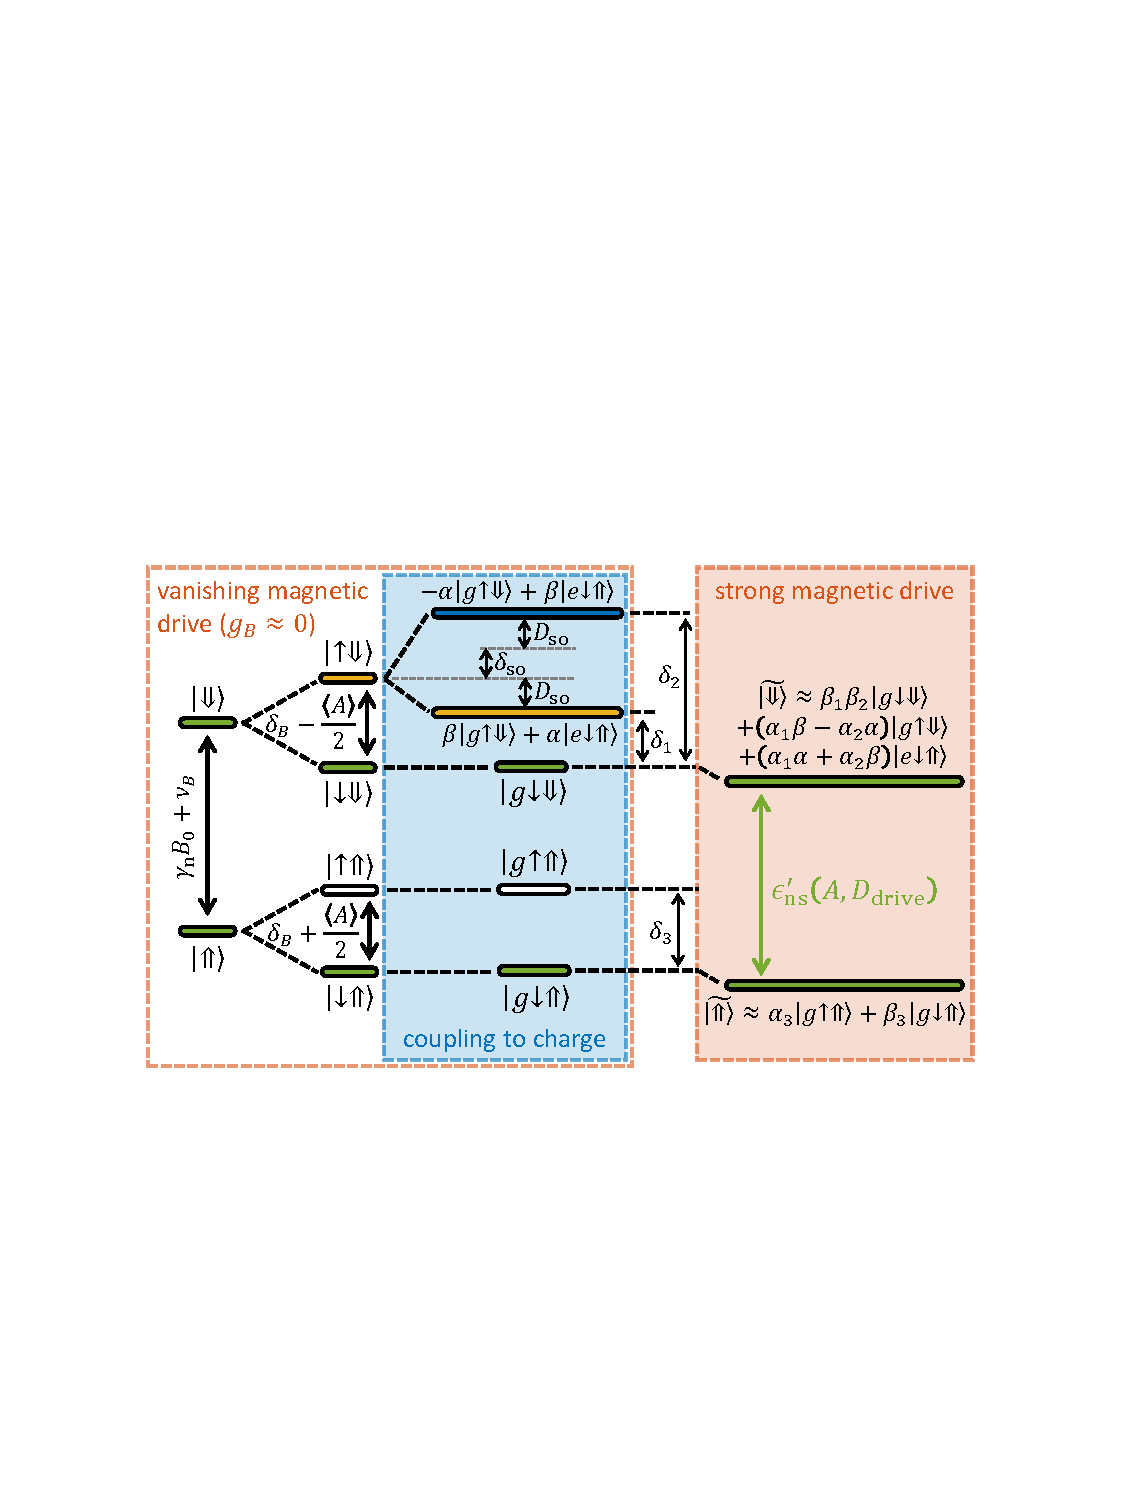
\includegraphics[width=\columnwidth]{fig2_levels}
	\caption[Nuclear spin level diagram with a strong magnetic drive]{\textbf{Nuclear spin level diagram with a strong magnetic drive}
 		Nuclear spin levels in the rotating frame of the magnetic drive $B_{\rm ac}$ at frequency $\nu_B$. From left to right, the system eigenstates are shown while adding the electron spin state, then the charge state, then increasing the strength of the magnetic drive. See main text for a detailed description.}
	\label{fig:levels}
\end{figure}

We now show that, by adopting a different choice of device tuning, the nuclear spin can be made largely insensitive to electrical noise, while having its electric dipole transition increased even further. This is achieved by tuning the charge qubit in resonance with the flip-flop qubit ($\epsilon_{\rm o} \approx \epsilon_{\rm ff}$, i.e. $\delta_{\rm so}\approx 0$), the magnetic drive in resonance with the electron spin ($\delta_B = \gamma_eB_0 - \langle A \rangle /2 -\nu_B\approx 0$), and the electric drive in resonance with the flip-flop (and charge) qubit ($\delta_E \approx 0$). In this strongly hybridized regime, second-order perturbation theory can not be directly applied. We therefore analyze the nuclear spin Hamiltonian $H_{\rm ns}$ by expressing it in the rotating frame of the magnetic drive by using the transformation:
\begin{subequations}
\begin{equation}
\mathcal{H}'=U^\dagger\mathcal{H}_{ns}U-i\hbar U\dot{U}^\dagger,
\end{equation}
\begin{equation}
U=e^{i2\pi\nu_Bt\left(S_z+I_z\right)}.
\end{equation}
\end{subequations}
We get

\begin{equation}
i\hbar U\dot{U}^\dagger=h\nu_B\left(S_z-I_z\right)
\end{equation}

and with $\cos(2\pi\nu_B t)=\frac{1}{2}\left(e^{i2\nu_B t}+e^{-i2\nu_B t}\right)$ follows

\begin{equation}
UH_{\rm ESR}U^\dagger=\frac{B_{\rm ac}}{2}\left[\gamma_e
\begin{pmatrix}
0 & e^{2\cdot i2\pi\nu_Bt}+1\\
e^{-2\cdot i2\pi\nu_Bt}+1 & 0
\end{pmatrix}-
\gamma_n\begin{pmatrix}
0 & e^{2\cdot i2\pi\nu_Bt}+1\\
e^{-2\cdot i2\pi\nu_Bt}+1 & 0
\end{pmatrix}\right]
\end{equation}

We neglect the counter-rotating terms, according to the rotating wave approximation and arrive at the transformed Hamiltonian of 

\begin{multline} \label{eq:H_nsRot}
\mathcal{H}'=\underbrace{\left(\gamma_e B_0 - \nu_B\right)}_{\delta_B}S_z-(\gamma_nB_0+\nu_B)I_z\\
+\frac{B_{ac}}{2}\left(\gamma_eS_x-\gamma_nI_x\right)+\mathcal{H}_{\rm orb}+\mathcal{H}_A^{\rm orb}+\mathcal{H}_E,
\end{multline}

where the magnetic drive is time-independent. 

The dominant energy scale in the above Hamiltonian is given by the term $-(\gamma_nB_0+\nu_B)I_z$, which represents the energy splitting of the nuclear spin states, but shifted to microwave frequencies by the transformation to the rotating frame of $\mathcal{H}_{\rm ESR}$. The corresponding energy levels are shown as $\ket{\Uparrow}, \ket{\Downarrow}$ at the left-most end of Fig.~\ref{fig:levels}. These levels are further split by the electron spin Hamiltonian, $\left(\delta_B+\langle A\rangle I_z\right)S_z+2g_BS_x$, where the expectation value of the hyperfine coupling $\langle A\rangle$ depends on the electron charge state, yielding the electron-nuclear spin levels shown in Fig. \ref{fig:levels}, depicted in the limit of vanishing $B_{\rm ac}$ (and therefore $g_B$) (see Fig. \ref{fig:hybridlevels}). In this case, the nuclear-spin transition frequency, in the rotating frame, with the electron in the ground state, is:

\begin{equation} \label{eq:e_ns}
\epsilon'_{\rm ns}(A) = \gamma_nB_0 + \nu_B + \langle A\rangle/2.
\end{equation}

\begin{figure}
\centering
	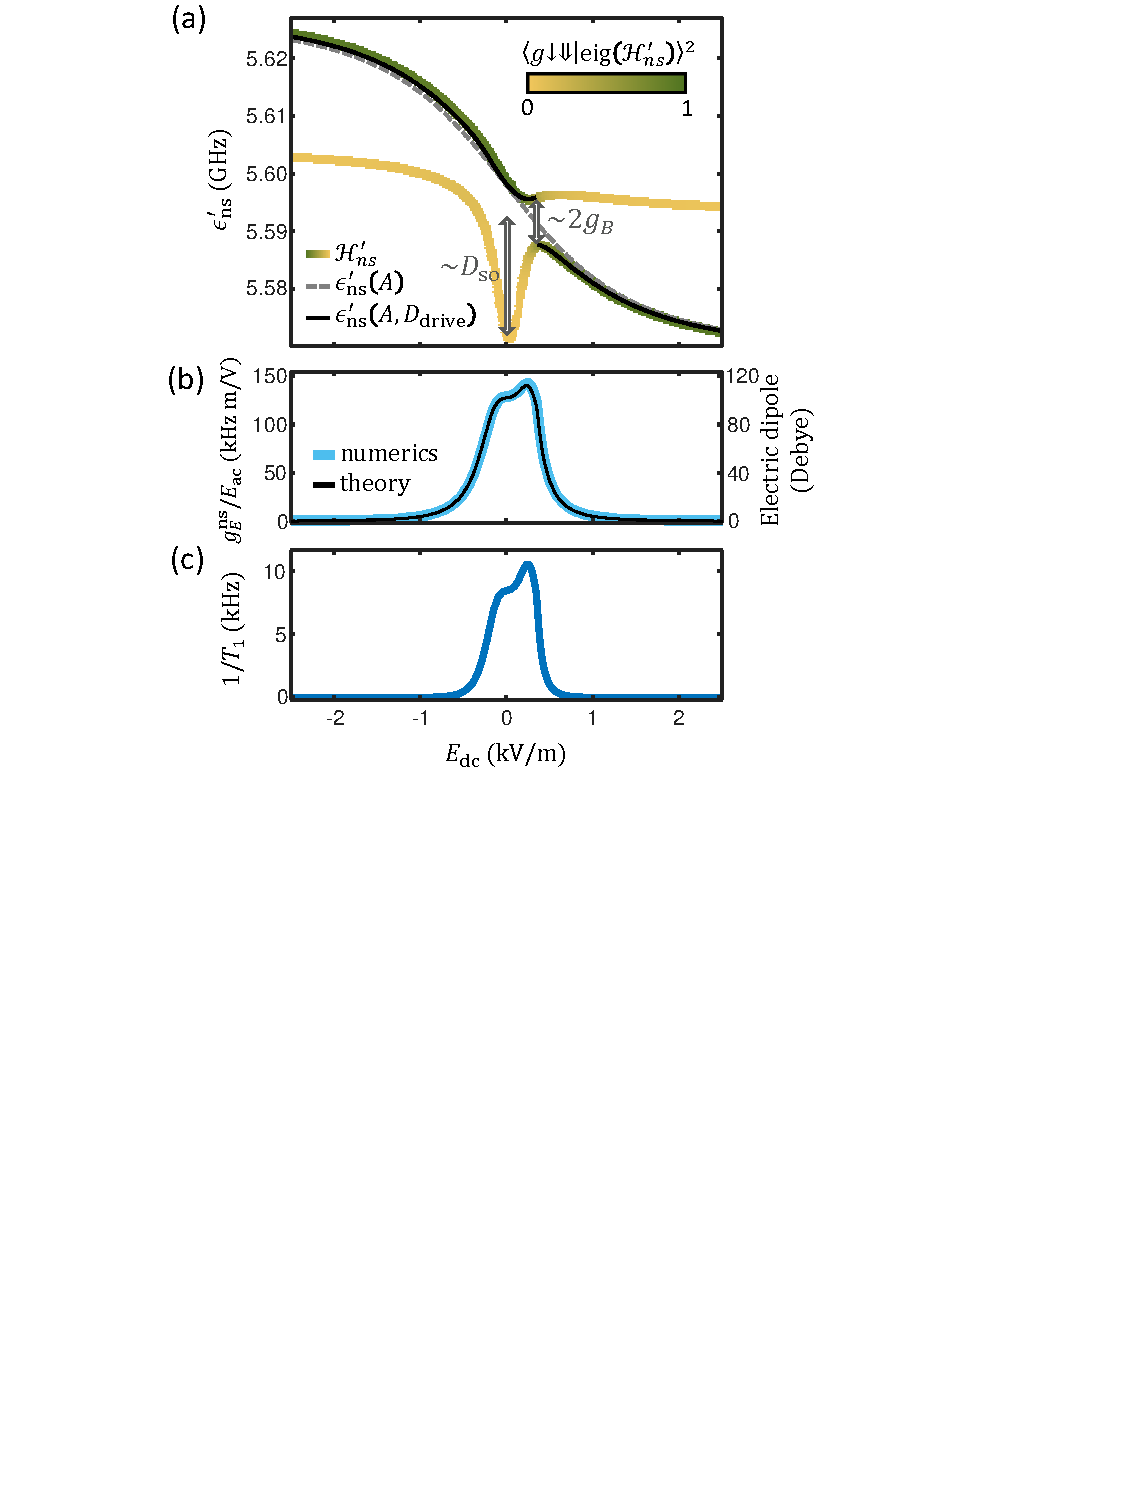
\includegraphics[width=0.9\columnwidth]{fig3_clock_v2}
	\caption[Nuclear qubit dispersion, dipole strength and relaxation]{
	\textbf{Nuclear qubit dispersion, dipole strength and relaxation. a}, Nuclear spin transition frequency $\epsilon'_{\rm ns}$ in the rotating frame of the magnetic drive $B_{\rm ac}$, as a function of the static vertical electric field $E_{\rm dc}$ across the donor-dot system, for vanishing magnetic drive ($\epsilon'_{\rm ns}(A)$ -- Eq.~\ref{eq:e_ns}, grey dashed line) and strong magnetic drive ($\epsilon'_{\rm ns}(A,D_{\rm drive})$ -- Eq.~\ref{eq:e_ns_Ddrive}, black solid line). We have assumed $B_0=0.2$~T, $B_{\rm ac}=0.6$~mT, $d=15$~nm and $V_t\approx \epsilon_{\rm ff}$ and $\nu_B\approx\gamma_eB_0-A/4$ (since $\langle A \rangle = A/2$ at the ionization point). Green/yellow lines show transition frequencies calculated numerically from the Hamiltonian in Eq. \ref{eq:H_nsRot}. The color indicates the degree of admixture of the bare $\ket{g\downarrow\Downarrow}$ state into the higher $\mathcal{H}'_{ns}$ eigenstate corresponding to each transition. The nuclear spin transition (predominantly $\ket{g\downarrow\Uparrow}\leftrightarrow\ket{g\downarrow\Downarrow}$, green) anticrosses a flip-flop transition (predominantly $\ket{g\downarrow\Uparrow}\leftrightarrow\ket{g\uparrow\Downarrow}$, yellow) at $E_{\rm dc}=350$~V/m, with a splitting $\sim2g_B$ set by the strength of the magnetic drive. The flip-flop transition is strongly shifted by $D_{\rm so}$, due to its coupling to the charge qubit states around $E_{\rm dc}=0$. At $E_{\rm dc}=250$~V/m, the nuclear-spin excited eigenstate has $\sim75\%$ of $\ket{g\downarrow\Downarrow}$ and is robust against electrical noise ($\partial\epsilon'_{\rm ns}/\partial E_{\rm dc}=0$).
	\textbf{b} Nuclear electric dipole strength $p_E^{\rm ns}=\partial g_E^{\rm ns} / \partial E_{\rm ac}$ obtained from Eqs.~\ref{eq:g_E^ns} (theory, black line), or for numerical diagonalization of the full Hamiltonian $\mathcal{H}'$ under $E_{\rm ac}$ drive (numerics, light blue line). For the choice of parameters used in this figure,  $p_E^{\rm ns}$ peaks where $E_{\rm dc}=250$~V/m. 
		\textbf{c} Nuclear spin relaxation rate $1/T_{\rm 1,ns}$ in the presence of the magnetic drive $B_{\rm ac}$ and the effect of coupling to phonons via charge states, Eq.~\ref{eq:T1ff}.
	}
	\label{fig:clock}
\end{figure}

In Fig. \ref{fig:clock}a we plot $\epsilon'_{\rm ns}(A)$ (dashed line) by including the dependence of $\langle A \rangle$ on vertical electric field $E_{\rm dc}$ (from Eqs.~\eqref{eq:H_orb},\eqref{eq:H_A}). This is valid when the electron charge states are far detuned from the spin levels ($\delta_{\rm so}\gg g_{\rm so}$). The plot highlights the strong dependence of $\epsilon'_{\rm ns}$ on electric fields under such conditions. 

However, the nuclear spin dispersion changes dramatically when $\delta_{\rm so}$ approaches zero. In that case, $\mathcal{H}_A^{\rm orb}$ hybridizes the flip-flop and charge states, as shown in the blue panel within Fig. \ref{fig:levels}. The overall ground state is $\ket{g\downarrow\Uparrow}$, but the excited flip-flop state splits into two hybridized states $\beta \ket{g\uparrow\Downarrow}+ \alpha\ket{e\downarrow\Uparrow}$ and $-\alpha \ket{g\uparrow\Downarrow} + \beta\ket{e\downarrow\Uparrow}$, with:

\begin{subequations} \label{eq:alphabeta}
\begin{eqnarray}
\alpha=\frac{\theta}{\sqrt{\theta^2+1}},~~~\theta=\frac{\delta_{\rm so}-\sqrt{{\delta_{\rm so}}^2+4{g_{\rm so}}^2}}{2g_{\rm so}},
\end{eqnarray}
\begin{eqnarray}
\beta=\frac{\phi}{\sqrt{\phi^2+1}},~~~\phi=\frac{\delta_{\rm so}+\sqrt{{\delta_{\rm so}}^2+4{g_{\rm so}}^2}}{2g_{\rm so}},
\end{eqnarray}
\end{subequations}
so that $\alpha=\beta=1/\sqrt{2}$ for $\delta_{\rm so}=0$ (as Eq. \eqref{eq:ff_hybrid}). 

As a final step, by increasing the magnetic drive amplitude $B_{\rm ac}$, the Hamiltonian term $2g_BS_x$ couples the electron spin $\ket{\uparrow}$ and $\ket{\downarrow}$ states, further hybridizing the system eigenstates $\ket{g\downarrow\Downarrow}$ with the hybridized flip-flop states as well as $\ket{g\uparrow\Uparrow}$. Two of those eigenstates, which we call $\widetilde{\ket{\Downarrow}}$ and $\widetilde{\ket{\Uparrow}}$ (Fig.~\ref{fig:levels}, orange box), are chiefly composed of the tensor product of the nuclear $\ket{\Downarrow}$, $\ket{\Uparrow}$ states with the ground charge state $\ket{g}$ and the ground $\ket{\downarrow}$ electron spin state. They are obtained as:

\begin{eqnarray} \label{eq:tildestates}
\widetilde{\ket{\Downarrow}} & \approx & \beta_1 \beta_2\ket{g\downarrow\Downarrow} + \left(\alpha_1 \beta - \alpha_2 \alpha\right) \ket{g\uparrow\Downarrow} + (\alpha_1 \alpha + \alpha_2 \beta)\ket{e\downarrow\Uparrow}\\
\widetilde{\ket{\Uparrow}}&\approx & \alpha_3 \ket{g\uparrow\Uparrow} + \beta_3\ket{g\downarrow\Uparrow},
\end{eqnarray}
with coefficients $\alpha_i, \beta_i$ ($i=1,2,3$) given by:

\begin{subequations} \label{eq:alphaibetai}
\begin{equation} \label{eq:alpha1}
\alpha_1=\frac{\theta_1}{\sqrt{{\theta_1}^2+1}},~~~
\theta_1=\frac{\delta_1-\sqrt{{\delta_1}^2+(2{\beta g_B})^2}}{2\beta g_B}
\end{equation}
\begin{equation} \label{eq:beta1}
\beta_1=\frac{\phi_1}{\sqrt{{\phi_1}^2+1}},~~~
\phi_1=\frac{\delta_1+\sqrt{{\delta_1}^2+(2{\beta g_B})^2}}{2\beta g_B}
\end{equation}
\begin{equation} \label{eq:alpha2}
\alpha_2=\frac{\theta_2}{\sqrt{{\theta_2}^2+1}},~~~
\theta_2=\frac{\delta_2-\sqrt{{\delta_2}^2+(2\alpha g_B)^2}}{2\alpha g_B}
\end{equation}
\begin{equation} \label{eq:beta2}
\beta_2=\frac{\phi_2}{\sqrt{{\phi_2}^2+1}},~~~
\phi_2=\frac{\delta_2+\sqrt{{\delta_2}^2+(2{\alpha g_B})^2}}{2\alpha g_B}
\end{equation}
\begin{equation} \label{eq:alpha3}
\alpha_3=\frac{\theta_3}{\sqrt{{\theta_3}^2+1}},~~~
\theta_3=\frac{\delta_3-\sqrt{{\delta_3}^2+4{g_B}^2}}{2g_B}
\end{equation}
\begin{equation} \label{eq:beta3}
\beta_3=\frac{\phi_3}{\sqrt{{\phi_3}^2+1}},~~~
\phi_3=\frac{\delta_3+\sqrt{{\delta_3}^2+4{g_B}^2}}{2g_B}
\end{equation}
\end{subequations}

The energy splitting between $\widetilde{\ket{\Downarrow}}$ and $\widetilde{\ket{\Uparrow}}$, $\epsilon'_{\rm ns}$, equals the bare nuclear-spin transition, $\epsilon'_{\rm ns}(A)$ (Eq.~\eqref{eq:e_ns}), plus an amount that dependents on $E_{\rm dc}$:

\begin{equation} \label{eq:e_ns_Ddrive}
\epsilon'_{\rm ns}(A,D_{\rm drive})=\epsilon'_{\rm ns}(A)-D_{\rm drive}(E_{\rm dc}),
\end{equation}
where $D_{\rm drive}$ is an AC-Stark shift given by second order perturbation theory to (analogous to Eqs. \eqref{eq:Dorb}, \eqref{eq:Ddd}):
\begin{subequations}
\begin{equation} \label{eq:Ddrive}
D_{\rm drive}(E_{\rm dc})=\sum_{i=1,2,3}\frac{\delta_i}{2}\left(\sqrt{1+\left(\frac{2g_i}{\delta_i}\right)^2}-1\right),
\end{equation}
\begin{equation} \label{eq:g_alpha_beta}
g_1=\beta g_B,~~~~g_2=-\alpha g_B,~~~~g_3=g_B.
\end{equation}
\end{subequations}

This equation agrees with numerical simulations of the full Hamiltonian in the rotating frame of Eq.~\eqref{eq:H_nsRot} (Fig. \ref{fig:clock}a). Around the ionization point, the flip-flop transition (itself strongly affected by the hybridization with the charge state) anticrosses the nuclear spin transition (in the rotating frame), creating a region where $\partial\epsilon'_{\rm ns}/\partial E_{\rm dc}=0$, i.e. a first-order `clock transition' \cite{Bollinger1985,Wolfowicz2013} where $\epsilon'_{\rm ns}$ is insensitive to electric noise to first order. Further adjustment of the parameters allows for $\partial^2\epsilon'_{\rm ns}/\partial {E_{\rm dc}}^2=0$ (second-order clock transition), improving noise insensitivity even further.

In a key result of our proposal, the small admixture of the excited charge state, $\ket{e}$, into $\widetilde{\ket{\Downarrow}}$ creates an electric-dipole transition for the nuclear spin. Indeed, the $\widetilde{\ket{\Downarrow}} \leftrightarrow \widetilde{\ket{\Uparrow}}$ transition can be electrically-driven at a rate given by the charge admixture coefficients in Eq.~\ref{eq:alphaibetai} (see also Fig.~\ref{fig:clock}b):

\begin{equation} \label{eq:g_E^ns}
g_{E}^{\rm ns}=g_E\beta_3\left(\alpha_1\alpha+\alpha_2\beta\right),
\end{equation}

This electric dipole transition, at microwave frequencies, can reach $>100$~Debye around $E_{\rm dc}=0$ (Fig.~\ref{fig:clock}b). This means that even an extremely weak AC electric field, $E_{\rm ac}\approx 3$~V/m, can drive a nuclear spin transition at a MHz Rabi frequency. This is two orders of magnitude faster than the typical Rabi frequencies obtained with standard (NMR) magnetic drive at radiofrequency \cite{Pla2013}, and an order of magnitude faster than obtained (at very high electric drive amplitudes) in a recent experiment where electrically-driven NMR was achieved by modulating the quantization axis of the electron spin \cite{Sigillito2017}.

\subsection{Resilience against charge noise}

The issue of charge noise is of paramount importance in semiconductor spin qubits. It is known, experimentally and theoretically, that charge fluctuators yield a $1/\nu$ frequency dependence of the noise spectral density \cite{Paladino2014}. These models capture the averaged collective effect of many charge fluctuators on the qubit operation. In this case, charge noise results in a slow drift of the qubit electrostatic environment. Indeed, since individual qubit operations take less than a microsecond, the qubit environment is usually static within a single operations, but fluctuates in between operations. The estimating the noise in our system based on experimental results yields is 1.7~${\mu \rm eV}$ r.m.s. noise amplitude, which, given the distance between donor and interface $d \approx 15$~nm, corresponds to an r.m.s. noise on the amplitude of the vertical electric field of order 100~V/m (see chapter \ref{sec:noise}). Inserting this into our model of the qubit energy according to Eq. \eqref{eq:dephasing_rate} yields a predicted nuclear spin dephasing rate of order $1-10$~kHz. Note that, similarly to dressed states \cite{London2013,Laucht2016,Laucht2016a}, the addition of the strong magnetic drive has the effect of extending the coherence of our qubit. However, here the suppressed noise is of electrical nature (despite the drive being magnetic), given the particular hybridization with charge states.

We thus derived the striking result that the nuclear spin has a strong electric dipole despite being robust against electrical noise. This is because, while the qubit precession frequency is insensitive to noise, its effective transverse matrix element is strongly dependent on electric fields. Importantly, the electric dipole is induced on the nuclear spin  only around the flip-flop transition frequency, which is at several GHz. Since the charge and gate noise in nanoscale devices mainly has a $1/\nu$ spectrum, the power spectral density of the noise at the frequency that would affect the nuclear qubit is expected to be very weak. Moreover, at the same bias point where the CT ($\partial\epsilon'_{\rm ns}/\partial E_{\rm dc}=0$) for the nuclear energy takes place, the nuclear electric dipole itself is also first-order insensitive to electrical noise, since $\partial g_{E}^{\rm ns}/\partial E_{\rm dc}=0$ (Fig. \ref{fig:clock}b). A realistic $1.5~\mu$eV charge detuning noise \cite{Freeman2017} would make $g_{E}^{\rm ns}$ fluctuate by only $\sim2\%$. In other words, in this system both the free precession frequency and the Rabi frequency can be made first-order insensitive to charge noise.

As a final note, although we assumed $\delta_{\rm so} \rightarrow 0$, the electric and magnetic driving fields are still off-resonance with the eigenstates of the full Hamiltonian $\mathcal{H}_{\rm ns}$ due to the hybridized charge-flip-flop states, ensuring minimal excitation of the $\ket{\uparrow}$ and $\ket{e}$ states.

\subsection{Coupling to microwave cavity photons}

This strong electric dipole at microwave frequencies provides a pathway for strongly coupling $^{31}$P nuclear spins to microwave resonators \cite{Blais2004}, where a vacuum field $E_{\rm vac}$ of a few V/m can result in vacuum Rabi splittings around 1~MHz. This could be achieved \textit{e.g.} by connecting the top blue gate on Fig.~\ref{fig:Raman}a to the center pin of a superconducting coplanar waveguide resonator. Our proposal thus provides a solution to the fact that the standard (NMR) nuclear-spin transition does not naturally couple to microwave resonators. Similarly to other proposals  \cite{Pachos2002,Childress2004,Feng2008,Abanto2010}, here it is a classical drive ($B_{\rm ac}$) that enables coupling to a quantum field ($E_{\rm vac}$).

\subsection{Nuclear spin relaxation}

The engineered nuclear electric dipole also opens up a new pathway for nuclear spin relaxation: $\widetilde{\ket{\Downarrow}}$ can decay into $\widetilde{\ket{\Uparrow}}$ through a peculiar effect, where a photon from the driving field is combined with the nuclear spin energy (which is at radiofrequency) to emit a phonon at microwave frequency. The rate for this process can be roughly estimated as the admixture of the $\ket{e}$ charge excited state into the $\widetilde{\ket{\Downarrow}}$ eigenstate times the charge relaxation rate ${1}/{T_{1,\rm o}}$:

\begin{equation}\label{eq:T1ff}
\frac{1}{T_{1,\rm ns}}=\frac{|\widetilde{\bra{\Downarrow}}e\rangle|^2}{T_{1,\rm c}}\approx \frac{|\alpha_1\alpha+\alpha_2\beta|^2}{{T_{1,\rm c}}},
\end{equation}

where ${1}/{T_{1,\rm c}}=\Theta\epsilon_{\rm o}{V_t}^2$ (Ref.~\cite{Boross2016}), with $\Theta\approx2.37\times10^{-24}~{\rm s}^2$ determined by the silicon crystal properties. 

As Fig.~\ref{fig:clock}c shows, ${1}/{T_{1,\rm ns}}$ peaks, around the ionization point, at a value that is still two orders of magnitude slower than e.g. the spin's coupling rate to a microwave resonator, therefore allowing the strong coupling regime to be well within reach.


\subsection{Dependence of electric dipole strength and spin relaxation rate on frequency and field detuning} \label{supp:detdep}

In Fig.~\ref{fig:clock} we have shown an operation point ($E_{\rm dc}=250$~V/m and $\nu_B=5.565$~GHz) where the proposed nuclear spin electric dipole transition is robust against noise, i.e. both its precession frequency, $\epsilon_{\rm ns}'$, and electric dipole strength, $p^E_{\rm ns}=g_E^{\rm ns}/E_{\rm ac}$, are to first order insensitive to small perturbations of the static electric field. To understand how the system behaves when slightly detuned from the optimal working point, we calculate the dependence of the nuclear spin electric dipole strength $p^E_{\rm ns}$ and relaxation rate $1/T_{1, \rm ns}$ on the magnetic drive frequency, $\nu_B$, and on the static electric field, $E_{\rm dc}$. 

\begin{figure}
	\centering
	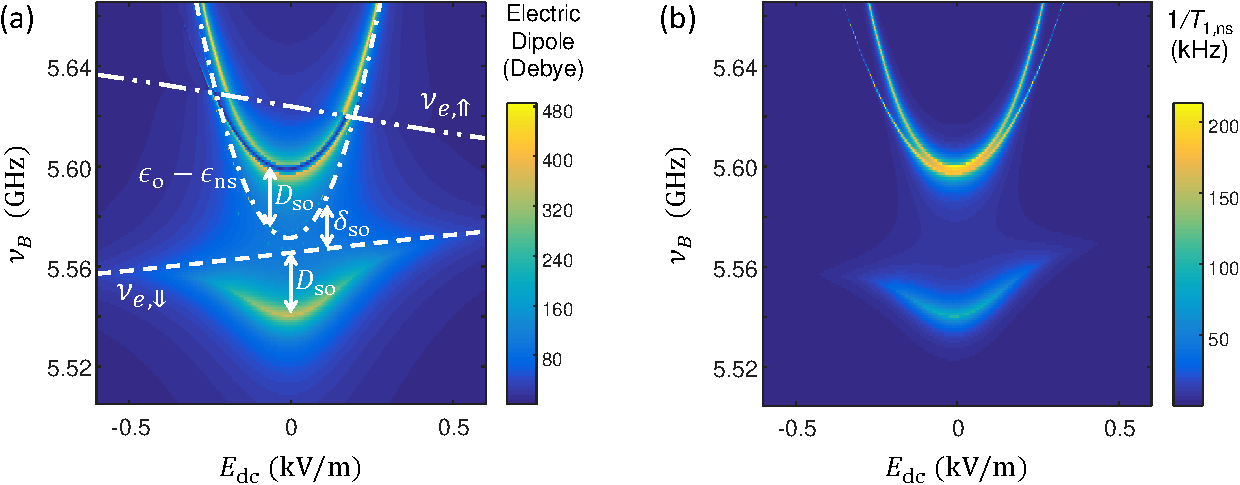
\includegraphics[width=1\textwidth]{fig4_v2}
	\caption[Nuclear electric dipole strength and relaxation as a function of electric field]{\textbf{Nuclear electric dipole strength and relaxation as a function of electric field. a},
	 Nuclear electric dipole strength $p_E^{\rm ns}$ and
		\textbf{b} nuclear spin relaxation rate $1/T_{\rm 1,ns}$, as a function of the donor-dot electric field detuning, $E_{\rm dc}$, and the magnetic drive frequency, $\nu_B$. $E_{\rm dc}=0$ is the ionization point. In \textbf{a}, the dashed line shows the ESR frequency $\nu_{e,\Downarrow}$ when the nuclear spin is in the  $\ket{\Downarrow}$ state, the dot-dashed line shows the charge qubit frequency minus the nuclear spin frequency, $\epsilon_{\rm o} - \epsilon_{\rm ns}$, and the dot-dot-dashed line the electron spin resonance frequency $\nu_{e,\Uparrow}$ when the nuclear spin is in the $\ket{\Uparrow}$ state. The charge and flip-flop states are detuned by $\delta_{\rm so}$, which is close to zero at $E_{\rm dc}=0$. Charge and flip-flop states then hybridize, shifting the system eigenenergies by an AC-Stark shift $D_{\rm so}$. The plots in Figs.~\ref{fig:clock}b,c correspond to specific line cuts of the graphs shown here, for $\nu_B=\nu_{e,\Downarrow}$ at $E_{\rm dc}=0$, \textit{i.e.} $\nu_B=5.565$~GHz.
	}
	\label{fig:fig4}
\end{figure}

The results are plotted in Fig. \ref{fig:fig4}. Both plots show two branches (bright yellow) where both dipole moment and relaxation rate are enhanced. To understand these branches, we refer to the level diagrams in Figs. \ref{fig:Raman}b,c. First, note that $\nu_B$ unequivocally sets the electric dipole transition frequency $\nu_E$ (in the simplest case, $\nu_E=\nu_B+\epsilon_{\rm ns}$). The two bright branches in  Fig.~\ref{fig:fig4}a,b correspond to $\nu_E$ being in resonance with either of the two charge-flip-flop hybridized states (yellow and blue states inside the light blue rectangle in Fig. \ref{fig:levels}). If the charge and flip-flop states were uncoupled or off-resonance, then the lower branch would simply correspond to the flip-flop dipole transition, $\nu_E=\nu_{e,\Downarrow}+\epsilon_{\rm ns}$ (where $\nu_{e,\Downarrow}$ is the electron spin resonance frequency when the nuclear spin is in the `down' state), which means that the magnetic drive frequency simply coincides with the electron spin resonance $\nu_B=\nu_{e,\Downarrow}$. This would represent a simple, on-resonance Raman transition, i.e. as in the sketch in Fig.~\ref{fig:Raman}b but where $\delta=0$. Then, the upper branches in Fig.~\ref{fig:fig4} would correspond to the pure charge transition, $\nu_E=\epsilon_{\rm o}$, or equivalently $\nu_B=\epsilon_{\rm o}-\epsilon_{\rm ns}$. However, since the charge and flip-flop states are coupled, they hybridize and further split the two branches by an amount equal to $D_{\rm so}$.

Upon closer inspection, the upper branch shows an extra subtle feature. This branch corresponds to excitation conditions that put the magnetic drive frequency close to the electron spin resonance frequency when the nuclear spin is in the $\ket{\Uparrow}$ state, $\nu_{e,\Uparrow}$. This, in turn, creates a pair of dressed electron spin states that further split the upper branch into two, separated by the ESR (magnetic) Rabi frequency of the $\nu_{e,\Uparrow}$ resonance. 

\section{Long-distance coupling of nuclear spin qubits} \label{sec:long}

\begin{figure}
\centering
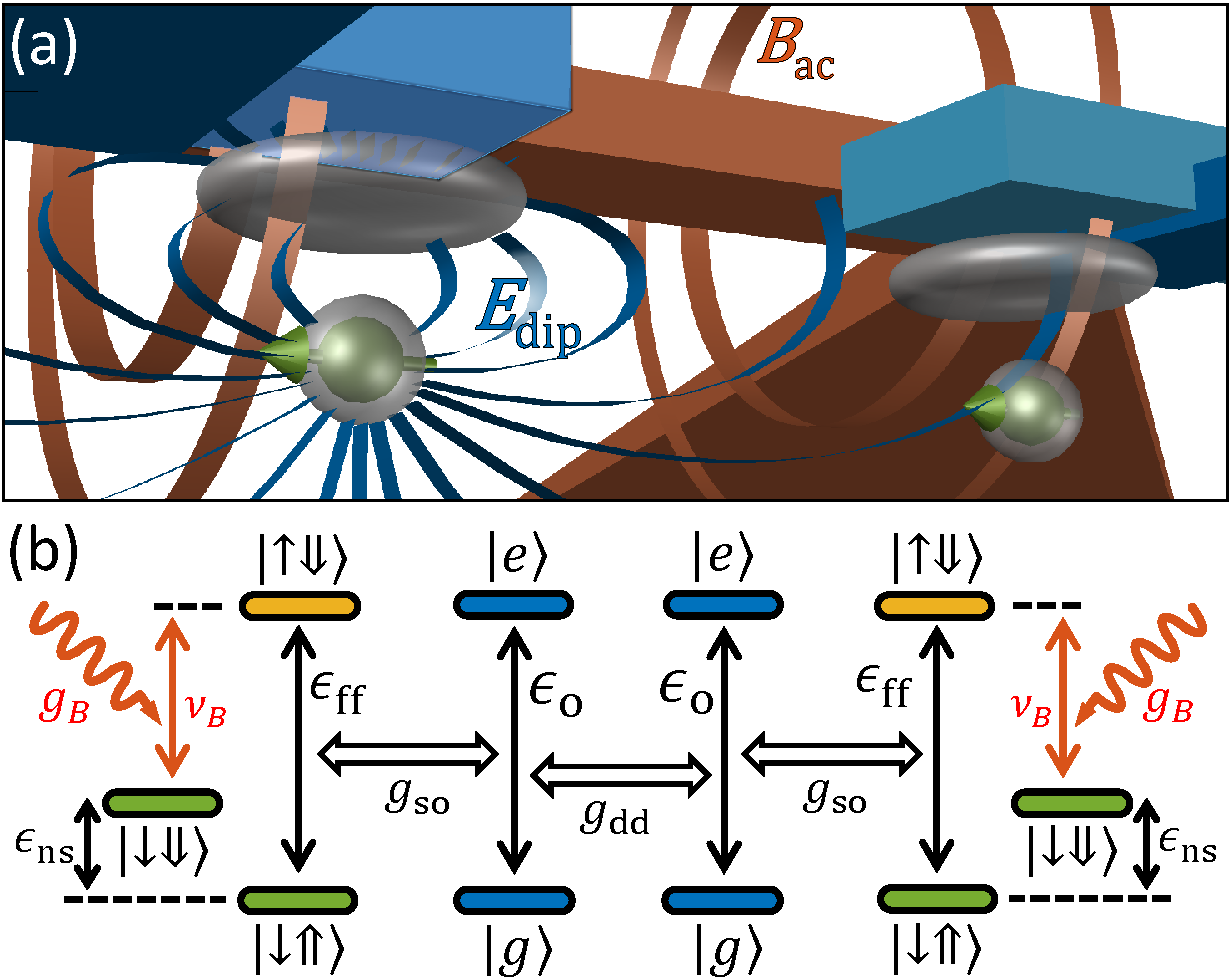
\includegraphics[width=0.9\columnwidth]{fig5_2-qubit_nuc}
\caption[Long distance coupling of two nuclear qubits]{
\textbf{Long distance coupling of two nuclear qubits. a}, Components and \textbf{b} level diagram for long-distance coupling of two $^{31}$P nuclear spins via electric dipole-dipole interactions. Each displaced electron produces an electric dipole field $E_{\rm dip}$ (shown only for one electron). The charge dipoles induced by displacing the electron wavefunction partly towards the interface dot interact with a strength $g_{\rm dd}$ (Eq.~\ref{eq:g_dd}), and the charge qubits interact with the flip-flop states with strength $g_{\rm so}$ (Eq.~\ref{eq:g_so}). Adding the (global) magnetic drive of strength $g_B$ and tuning the system to the fully-hybridized regime described in Sec.~\ref{sec:robust} results in a nuclear-nuclear coupling strength $g_{\rm 2q}^{\rm ns} \approx 0.55$~MHz at a $400$~nm distance (Eq.~\ref{eq:nucSWAP}).
}
\label{fig:2-qubit_nuc}
\end{figure}

We have shown in the previous section that a robust electric dipole at microwave frequencies is induced on the nuclear spin by the magnetic drive $B_{\rm ac}$, combined with the spin-charge hybridization that is obtained by displacing the electron from the donor towards an interface quantum dot. A natural and important extension of this effect is to exploit the induced electric dipole to achieve a long-distance coupling of the nuclear spins, mediated by long-range electric dipole interaction, similar as for the flip flop qubit in chapter \ref{Chapter2}, as illustrated in Fig. \ref{fig:2-qubit_nuc}a \cite{Tosi2017}. This dipole interaction between the charge qubits results in a coupling of $g_dd$ (eq. \eqref{eq:g_dd}). 

Two distant nuclear spin qubits can then be coupled when both electrons are around their ionization point, and an AC magnetic drive $B_{\rm ac}$ is applied (Fig. \ref{fig:2-qubit_nuc}a,b) to each of them, resulting in the electric dipole $p_E^{\rm ns}$ at microwave frequencies. For the operation parameters used in Fig.~\ref{fig:clock}, $\epsilon_{\rm o}\approx\epsilon_{\rm ff}\approx\nu_B+\epsilon_{\rm ns}$ and $g_B\ll g_{\rm so}$, the two-qubit coupling rate is obtained, via second-order perturbation theory, as:

\begin{eqnarray} \label{eq:nucSWAP}
g_{\rm 2q}^{\rm ns} & = & \bra{\tilde{\Downarrow}_1 \tilde{\Uparrow}_2}\mathcal{H}_{\rm ns}\ket{\tilde{\Uparrow}_1 \tilde{\Downarrow}_2}\\
 & =& \left(\frac{g_B}{g_{\rm so}}\right)^2g_{\rm dd},
\end{eqnarray}
 
which is valid if $g_B\ll (g_{\rm so})^2/g_{\rm dd}$. For two nuclear spins $r=400$~nm apart, $g_{\rm 2q}^{\rm ns}=0.55$~MHz, yielding a $\sqrt{i\mathrm{SWAP}}$ gate time of $\sim230$~ns. To put this in perspective, the Kane's proposal \cite{Kane1998} described a system of  two $^{31}$P nuclear spins placed $r=15$~nm apart, where a $\sqrt{i\mathrm{SWAP}}$ gate mediated by the electron spin exchange interaction requires $3~\mu$s -- an order magnitude slower, for over an order of magnitude tighter spacing. A recent proposal by Hill et al. \cite{Hill2015} describes a CNOT gate between nuclear spins mediated by the electron magnetic dipole interaction, wherein the 2-qubit gate time requires 300~$\mu$s for donors spaced $30$~nm apart -- three orders of magnitude slower than the electric-dipole mediated gate we have introduced here.


This method of coupling nuclear spin qubits at long distances via their induced electric dipole can be switched off completely -- $p_E^{\rm ns} \approx 0$ when the electron charge is moved back to the donor -- thus offering great flexibility in how multi-qubit operations are undertaken in a large array of qubits. The magnetic drive $B_{\rm ac}$ necessary to induce the dipole can be a global, always-on field, acting on every donor in the array. This can be optimally achieved by placing the device in a three-dimensional microwave cavity with good $B_{\rm ac}$ homogeneity \cite{Angerer2016}. Alternatively, $B_{\rm ac}$ could be delivered locally using a grid of microwave striplines \cite{Li2018}. The ``robust'' mode of operation described in Sec.~\ref{sec:robust} requires $\delta_B \approx 0$, i.e. $B_{\rm ac}$ in resonance with the electron spin transition. However, this resonance condition must be met while the donor is at the ionization point, where the hyperfine coupling is approximately half the value it has while the electron is fully at the donor ($\langle A\rangle \approx A/2$), thus $\nu_B \approx \gamma_e B_0 - A/4$. Therefore, idle qubits with the electron resting at the donor will be left unaffected by the global magnetic drive, and completely decoupled from both electric and magnetic AC-fields.


\section{Conclusion} \label{sec:conclusion}

The exceptional quantum coherence of $^{31}$P nuclear spins in isotopically enriched $^{28}$Si is experimentally well established \cite{Saeedi2013,Muhonen2014}. However, it has been widely accepted that using the $^{31}$P nuclear spin as the physical qubit in a quantum computer architecture requires dealing with the very small nuclear magnetic dipole, which renders operation and multi-qubit coupling slow and cumbersome \cite{Kane1998,OGorman2016,Hill2015}, even with inter-donor spacings $\sim 10$~nm. Indeed, most of the recent focus on $^{31}$P nuclei for quantum information has been on using them as long-lived quantum memories \cite{Morton2008,Freer2017} rather than data qubits. 

By engineering an electric dipole transition, we have shown here that the $^{31}$P qubit can also be driven at microwave frequencies, and coupled to other nuclei or to microwave cavities via electric dipole interactions, thus making it also a convenient system as a data qubit. The effects of electrical noise can be strongly suppressed by operating around `clock transitions', which allow the $^{31}$P system to retain dephasing times in the $0.1 - 1$~ms range. The nuclear spin, equipped with an artificial electric dipole, can then be incorporated into large hybrid quantum architectures \cite{Xiang2012} where -- in analogy to flip-flop qubits \cite{Tosi2017} -- large arrays of nuclear qubits couple either by electric dipole-dipole coupling or via cavity microwave photons. In such architectures, the spacing between qubits can be several hundreds of nanometers, leaving ample space for classical interconnects \cite{Fisher2015,Franke2018} and readout devices, fabricated using conventional silicon nanoelectronics fabrication methods.